\chapter{Algoritmos e Operadores}
\label{ch:3_AlgoritmosOperadores}
Nesse trabalho procurou-se otimizar estratégias de produção através da busca pela localização ótima dos poços que compõem tais estratégias (mais detalhes na Seção \ref{sec:4_CasoEstudo}). Para a resolução desse problema, foram utilizados aqui os algoritmos genéticos. Tal escolha foi feita, principalmente, por conta da robustez destes algoritmos e de sua estrutura simples, o que permite a aplicações dos AGs em diversas situações. As versões clássicas do Algoritmo Genético Geracional e do Algoritmo Genético de Regime Permanente foram utilizadas nesse trabalho e serviram como base para versões modificadas do AG, que se adequaram melhor ao problema de DEP.

Quanto aos operadores de busca necessários para o bom desempenho do algoritmo, foram implementados operadores clássicos, encontrados na literatura, e proposto novos operadores que utilizam de conhecimento do problema para gerar soluções candidatas melhores. Por fim, também foram desenvolvidos duas versões de um operadores de busca local para refinar as soluções encontradas pelos AGs. As seções a seguir apresentam com mais detalhes a estrutura escolhida para representar as soluções candidatas; a função objetivo escolhida, a estrutura dos AGs clássicos e dos AGs modificados que foram implementados nesse trabalho; os operadores de seleção, recombinação e mutação desenvolvidos; o operador de busca local em conjunto com um novo operador que contabiliza o número de ocorrências das coordenadas de posição de cada poço da estratégia de produção; e, por fim, o tratamento de restrições adotadas.  

\section{Representação da Solução}
\label{sec:3_Representacao}
Cada indivíduo que compõe a população do algoritmo genético é uma estratégia de produção completa, que, por sua vez, aqui é representado por um conjunto de poços. Cada poço dessa estratégia é representado por um conjunto de sete variáveis de decisão, sendo elas:

\begin{itemize}

\item Posição, definida por três variáveis que representam as coordenadas I, J e K;
\item Direção do poço;
\item Largura do poço, correspondendo à quantidade de blocos que este ocupa na malha do modelo do reservatório; 
\item Tipo do poço (Produtor ou Injetor); e
\item Estado do poço (Aberto ou Fechado).

\end{itemize}

Apesar da “direção do poço”, da “largura do poço”, do “tipo do poço” e do “estado do poço” serem considerados para a representação do poço, estas variáveis não foram utilizadas no processo de otimização, tendo seus valores definidos a priori em conjunto com os engenheiros do grupo UNISIM. Além disso, a quantidade de cada tipo de poço também foi pré-determinada. 

Sendo assim, o número total de variáveis no processo de otimização vai depender da quantidade de poços definidos para a estratégia de produção: sendo N o número máximo de poços, a quantidade de variáveis a ser considerada será igual 3 $\times$ $N$. A Figura \ref{fig:fig3_1} apresenta o esquema de uma solução candidata de estratégia de produção a ser utilizada pelo algoritmo genético. Como pode ser visto na Figura \ref{fig:fig3_1}, cada indivíduo é representado, neste trabalho, por um vetor de valores discretos.

\begin{figure}[!htbp]
  \centering
  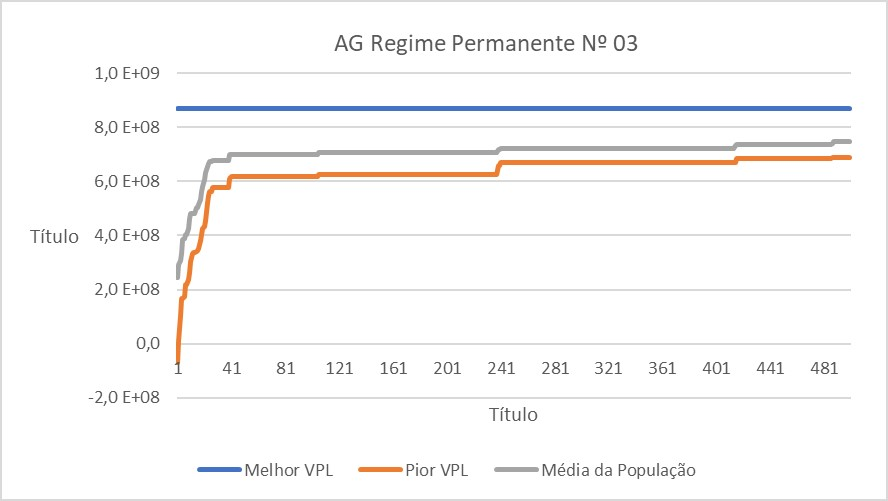
\includegraphics[scale=0.5]{3}
  \caption{Esquema da representação de uma solução candidata.}
  \label{fig:fig3_1}
\end{figure}

\section{Função Objetivo}
\label{sec:3_FuncaoObjetivo}
É comum o uso do Valor Presente Líquido para avaliar economicamente a viabilidade de uma dada estratégia de produção (conforme dito na Seção \ref{subsec:subsec:2_2_IndicadoresEconomicos}). Sendo assim, esse foi o indicador escolhido para avaliar as estratégias geradas pelos AGs implementados. Vale ressaltar que, para obter tal indicador, é necessária uma simulação de campo de petróleo e de ferramentas auxiliares para o cálculo do VPL (mais detalhes na Seção \ref{sec:4_FerramentasComputacionais}), sendo assim essa função objetivo é uma função de caixa preta. 

\section{Estrutura Geral dos Algoritmos Genéticos}

Tanto o Algoritmo Genético Geracional Clássico ($AG^{GC}$) quanto o Algoritmo Genético de Regime Permanente Clássico ($AG^{RPC}$) foram implementados nesse trabalho. No entanto, conforme o avanço dos experimentos realizados, alterações foram propostas para estes algoritmos, visando adequar os AGs aos novos operadores de busca propostos.  No total, foram três versões de AG utilizadas aqui.  As próximas seções apresentam com mais detalhes da estrutura das versões de AG aqui empregadas.

\subsection{Primeira versão}
\label{subsec:3_PrimeiraVersao}
A primeira versão consiste nas implementações clássicas tanto do AG Geracional quanto do AG de Regime Perante. Essa versão utiliza como base as implementações encontradas no \textit{framework} JMetal (mais detalhes na Seção \ref{sec:4_FerramentasComputacionais}).

\subsubsection{Algoritmo Genético Geracional Clássico}
\label{subsec:3_AlgoritmoGeneticoGeracionalClassico}
O Pseudocódigo \ref{alg:aggc} apresenta o AG Geracional encontrado no \textit{framework} JMetal. É possível notar que, apesar de uma população de novas soluções ser criada a cada iteração, o algoritmo implementado utiliza Elitismo. Essa versão do algoritmo substitui as duas piores soluções da população sucessora por duas das melhores soluções da população atual.

\begin{algorithm}[!htbp]
  \floatname{algorithm}{Pseudocódigo}
  \caption{Algoritmo Genético Geracional Clássico}
  \label{alg:aggc}
  \begin{algorithmic}
    \State Inicialize a população $P$ com $T$ soluções geradas aleatoriamente;
    \State Avalie as $N$ soluções da população $P$;
    \While{não for atingido o critério de parada }
      \For {$N$ vezes} \State:
        \State Selecione 2 soluções da população $P$;
        \State Aplique o operador de recombinação às soluções selecionadas;
        \State Aplique o operador de mutação à nova solução gerada;
        \State Avalie as novas soluções;
        \State Adicione as novas soluções à população sucessora $PS$;
      \EndFor
      \State Adicione as duas melhores soluções da população $P$ à população sucessora $PS$;
      \State Remova as duas piores soluções da população sucessora $PS$;
      \State Substitua a população $P$ pela população sucessora $PS$;
    \EndWhile
  \end{algorithmic}
\end{algorithm}

\subsubsection{Algoritmo Genético de Regime Permanente Clássico}
\label{subsec:3_AlgoritmoGeneticoRegimePermanente}
Como foi discutido na Seção \ref{subsec:2_1_ManutencaoPopulacao}, a estratégia de substituição é um aspecto importante do algoritmo genético de regime permanente. A versão do algoritmo encontrado no JMetal substitui a pior solução da população pela nova solução gerada, caso esta solução seja melhor. As etapas deste algoritmo são detalhadas no Pseudocódigo \ref{alg:agrpc}.

\begin{algorithm}[!htbp]
  \floatname{algorithm}{Pseudocódigo}
  \caption{Algoritmo Genético de Regime Permanente Clássico}
  \label{alg:agrpc}
  \begin{algorithmic}
    \State Inicialize a população $P$ com $T$ soluções geradas aleatoriamente;
    \State Avalie as $N$ soluções da população $P$;
    \While{não for atingido o critério de parada }
      \For {$N$ vezes} \State:
        \State Selecione 2 soluções da população $P$;
        \State Aplique o operador de recombinação às soluções selecionadas para gerar uma nova solução $i$;
        \State Aplique o operador de mutação à nova solução $i$;
        \State Avalie a nova solução $i$;
        \If{a nova solução $i$ for melhor que a pior solução da população $P$} 
          \State Substitua a pior solução da população pela nova solução $i$	
        \EndIf
      \EndFor
    \EndWhile
  \end{algorithmic}
\end{algorithm}

\subsection{Segunda Versão}
\label{sec:3_SegundaVersao}
Para a segunda versão, foi considerado somente o $AG^{RPC}$, uma vez que esse apresentou resultados melhores nos primeiros experimentos realizados (mais detalhes no Capítulo \ref{ch:5_ResultadosDiscucao}). 

A principal alteração feita foi em relação ao uso do operador de mutação. O $AG^{RPC}$, apresentado anteriormente, o operador de mutação é executado logo após a nova solução candidata ser criada pelo operador de recombinação. Aqui essa ordem foi alterada. Na versão proposta aqui, o operador é utilizado após a nova solução candidata ser avaliada, caso essa solução não seja boa o suficiente para ser incluída na população. Essa decisão foi tomada para adequar o AG ao operador de mutação que será descrito na Seção \ref{sec:3_OperadorMutacao} que, por utilizar o IEP para realizar alterações nas soluções, exige que a solução tenha sido avaliada previamente para que tais indicadores possam ser calculados. O Pseudocódigo \ref{alg:agrpm} apresenta todas as etapas do Alortimo Genético de Regime Permanente Modificado ($AG^{RPM}$).

\begin{algorithm}[!htbp]
  \floatname{algorithm}{Pseudocódigo}
  \caption{Algoritmo Genético de Regime Permanente Modificado}
  \label{alg:agrpm}
  \begin{algorithmic}
    \State Inicialize a população $P$ com $T$ soluções geradas aleatoriamente;
    \State Avalie as $N$ soluções da população $P$;
    \While{não for atingido o critério de parada }
      \For {$N$ vezes} \State:
        \State Selecione 2 soluções da população $P$;
        \State Aplique o operador de recombinação às soluções selecionadas para gerar uma nova solução $i$;
        \State Avalie a solução $i$;
        \If{a solução $i$ for melhor que a pior solução da população $P$} 
          \State Substitua a pior solução da população pela solução $i$	
        \Else
          \State Aplique o operador de mutação a solução $i$	
          \State Avalie novamente à solução $i$;
          \If{a solução $i$ for melhor que a pior solução da população $P$} 
            \State Substitua a pior solução da população pela solução $i$
          \EndIf
        \EndIf
      \EndFor
    \EndWhile
  \end{algorithmic}
\end{algorithm}

\subsection{Terceira Versão}
\label{sec:3_TerceiraVersao}
A segunda modificação feita ao AG foi para adicionar um novo operador para contar a quantidade de ocorrências de um valor as coordenadas I, J e K que definem a posição de um poço. Essa informação é utilizada, posteriormente, pelos operadores de recombinação e mutação, para gerar novas soluções privilegiando as coordenadas mais frequentes e que apresentaram melhores IEPs. Mais detalhes desse operador são apresentados na Seção \ref{sec:3_ContadorOcorrencias} desse capítulo. O Pseudocódigo \ref{alg:agrpm2} apresenta o AG com com tal operador ($AG^{CO}$).

\begin{algorithm}[!htbp]
  \floatname{algorithm}{Pseudocódigo}
  \caption{Algoritmo Genético de Regime Permanente com Contador de Ocorrências}
  \label{alg:agrpm2}
  \begin{algorithmic}
    \State Inicialize a população $P$ com $T$ soluções geradas aleatoriamente;
    \State Avalie as $N$ soluções da população $P$;
    \State Inicialize a contagem de ocorrências dos valores das coordenadas $I$, $J$ e $K$ de cada um dos poços da $N$ soluções da população $P$;
    \While{não for atingido o critério de parada }
      \For {$N$ vezes} \State:
        \State Selecione 2 soluções da população $P$;
        \State Aplique o operador de recombinação às soluções selecionadas para gerar uma nova solução $i$;
        \State Avalie a solução $i$;
        \If{a solução $i$ for melhor que a pior solução da população $P$} 
          \State Substitua a pior solução da população pela solução $i$	
          \State Atualize a contagem de ocorrências com os valores das coordenadas $I$, $J$ e $K$ de cada um dos poços da solução $i$;
        \Else
          \State Aplique o operador de mutação à solução $i$	
          \State Avalie novamente a solução $i$;
          \If{a solução $i$ for melhor que a pior solução da população $P$} 
            \State Substitua a pior solução da população pela solução $i$
            \State Atualize a contagem de ocorrências com os valores das coordenadas $I$, $J$ e $K$ de cada um dos poços da solução $i$;
          \EndIf
        \EndIf
      \EndFor
    \EndWhile
  \end{algorithmic}
\end{algorithm}

\section{Operador de Seleção}
\label{sec:3_OperadorSelecao}
O operador utilizado para a seleção das soluções é o de Seleção por Torneio Binário, que é uma variação do operador de Seleção por Torneio. Neste método de seleção, são escolhidos $k$ indivíduos da população para competir entre si e, então, o melhor dentre estes $k$ indivíduos é selecionado \cite{Kacprzyk2015}. Na Seleção por Torneio Binário, o valor de $k$ é igual a 2. A escolha por esse operador de seleção se deu por conta de sua facilidade de implementação e flexibilidade, já que é possível controlar a pressão seletiva através da quantidade $k$ de indivíduos que participarão do torneio, quanto maior o número de competidores, maior será a pressão seletiva \cite{Miller1995}.

\section{Operadores de Recombinação}
\label{sec:3_OperadorRecombinacao}
Os operadores de recombinação encontrados no \textit{framework} JMetal são voltados para tratar problemas de otimização em espaços contínuos (com codificação real), problemas de otimização combinatória (que utilizam codificações que correspondem a permutações de valores inteiros) e problemas que utilizam representação por cadeias binárias. Sendo assim, foram implementados aqui dois operadores de recombinação para tratar o problema de DEP. O primeiro operador escolhido é conhecido como Operador de Recombinação Uniforme, apresentado na Seção \ref{subsec:2_1_OperadorRecombinacao}, e seu funcionamento consiste basicamente em selecionar aleatoriamente cada elemento que comporá uma nova solução a partir dos elementos de uma das soluções pais escolhidos para o processo \cite{Talbi2009, Kacprzyk2015}.

O segundo operador foi implementado especificamente para esse problema.  Tal operador também gera uma nova solução candidata $O$ a partir de duas soluções candidatas EP1 e EP2. No entanto, os valores I, J e K de cada poço $p$ de $O$ são escolhidos de forma aleatória a partir de um conjunto de valores delimitados pelas coordenadas I, J e K do poço p de EP1 e EP2. Dessa forma os poços de EP1 e EP2 servem para limitar coordenadas dos poços de O. A Figura \ref{fig:fig3_2}, esquematiza a recombinação realizada por esse operador. No exemplo apresentado pela Figura \ref{fig:fig3_2}, a coordenada K do Poço da Nova solução O é 19, um valor escolhido aleatoriamente através do intervalo definido pela coordenada das soluções EP1 e EP2, nesse caso valores entre 18 e 22. A mesma lógica é aplicada as coordenadas I e J. O processo é então repetido para todos os poços que compõem a solução.

\begin{figure}[!htbp]
  \centering
  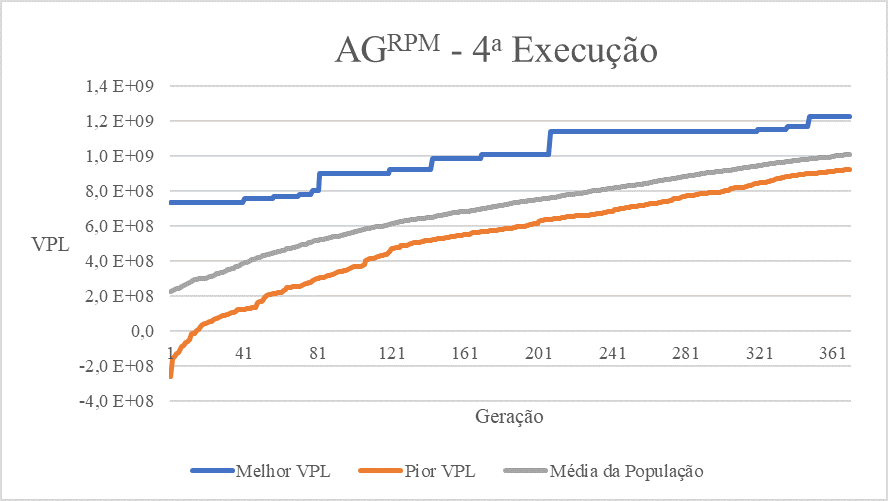
\includegraphics[scale=0.25]{4}
  \caption{Exemplo ilustrativo do operador de recombinação proposto para a resolução do problema de DEP.}
  \label{fig:fig3_2}
\end{figure}

\section{Operadores de Mutação}
\label{sec:3_OperadorMutacao}
Durante os experimentos realizados, dois operadores de mutação foram utilizados. O primeiro operador é conhecido por Mutação Pontual \cite{Kacprzyk2015}, voltado para utilização em algoritmos que adotam representações de valores discretos. Seu funcionamento consiste na alteração do valor de cada variável de um indivíduo, conforme uma probabilidade pré-definida, por outro valor dentro do conjunto de valores possíveis.

O segundo operador também aplica alterações aleatórias à posição de cada poço da estratégia de produção. No entanto a amplitude dessa alteração varia conforme a qualidade de cada poço, ou seja, quanto pior a qualidade de um dado poço, maior a variação que ele sofrerá durante a mutação. Para tal, é utilizado aqui o Indicador Econômico do Poço (IEP), apresentado na Seção \ref{subsec:2_2_IndicadoresPocos}. A amplitude da variação que é aplicada à localização do poço é calculada conforme a Equação \ref{eq:eq3_1}:

\begin{equation}
  \label{eq:eq3_1}
  a_i = 1 - \frac{IEP_m -IEP_i}{IEP_m -IEP_p}
\end{equation}

\noindent onde $a_i$ é a amplitude do poço $i$, $IEP_m$ o IEP do melhor poço, $IEP_p$ o IEP do pior poço e o $IEP_i$  o IEP do poço $i$ que está sendo alterado. Um detalhe importante sobre o cálculo da amplitude da variação é que, para um dado poço $i$ de uma solução $S$, o $IEP_m$ e o $IEP_p$, utilizados para o cálculo, são IEPs de poços de outras soluções que compõem a população do algoritmo. Tais poços são poços que respeitam a mesma restrição de localização do poço $i$. Essa decisão foi tomada por acreditar-se que não seria justo utilizar o IEP dos poços da mesma estratégia, uma vez que esses ocupam regiões diferentes e, consequentemente, têm IEPs distintos. Por fim, a componente aleatória desse operador fica por conta da escolha da direção para a qual o poço $i$ será deslocado com base na amplitude calculada.

\section{Operador de Busca Local}
\label{sec:3_OperadorBuscaLocal}
Como foi dito na Seção \ref{sec:2_1_MetaHeuristicas}, meta-heurísticas populacionais possuem uma boa capacidade de exploração do espaço de busca, no entanto não possuem uma boa capacidade de explotação. Tendo isso em mente, dois operadores de Busca Local são propostos aqui. O objetivo de tais operadores é realizar mudanças nos posicionamentos dos poços visando uma melhoria no VPL da estratégia de produção.

O primeiro operador, para cada poço de uma estratégia de produção, gera novas posições em sua vizinhança e desloca tal poço para a nova posição que levar aos maiores ganhos de VPL. Este processo é repetido, para o mesmo poço, até que não sejam geradas novas posições que levem a um aumento no VPL geral da estratégia de produção.

O segundo operador de busca local desenvolvido também procura deslocar cada poço da estratégia de produção para localizações que gerem maiores ganhos de VPL. No entanto, para tal operador essa abordagem foi refinada. Nessa segunda versão, para cada posição vizinha do poço é realizado uma avaliação e o poço tem sua posição alterada para a localização que proporcionar ganho no IEP desse poço. Caso nenhuma posição apresente um IEP melhor, é escolhida a posição que proporcione ganhos no VPL da solução, caso existam. 

\section{Contador de Ocorrências}
\label{sec:3_ContadorOcorrencias}  
Para a cada um dos poços que compõem uma estratégia de produção é possível definir um conjunto de valores I, J e K mínimos e máximos para limitar uma área no qual esses poços podem ser posicionados. O operador proposto aqui contabiliza a ocorrência dos valores do intervalo definido para cada uma das coordenadas. Tal informação é, posteriormente, utilizada pelos operadores de recombinação e mutação no momento de gerar valores aleatórios. Esse operador funciona de forma semelhante à Seleção por Roleta, utilizado para seleção de indivíduos pelo AG, onde indivíduos com fitness maiores têm mais chances de serem selecionados. No operador proposto aqui, os valores do intervalo de um eixo são escolhidos de forma aleatória, porém a probabilidade de escolha de um determinado valor é proporcional ao número de ocorrências desse valor. Dessa forma, espera-se que os valores com mais ocorrências sejam os mais promissores dentro do intervalo definido para um poço.

Entretanto, ainda pode acontecer de um valor do intervalo ser pouco promissor e ainda ter um alto número de ocorrências. Para contornar essa situação, é calculado um \textit{score} para cada valor de um dado intervalo. Esse cálculo leva em consideração a média do IEP obtido pelo poço e o número de ocorrências do valor dentro do intervalo de restrições do poço, conforme Equação \ref{eq:eq3_2}.

\begin{equation}
  \label{eq:eq3_2}
  S_{vi} = N_{vi} \times (\frac{IEP_{vi}}{IEP_{max}})
\end{equation}
  
sendo $S_{vi}$ o \textit{score} do valor $i$ de um dado intervalo, $N_{vi}$ o número de ocorrências do valor $i$ do dado intervalo, $IEP_{vi}$ a média do IEP obtido pelo valor $i$ do intervalo e o $IEP_{max}$, a maior média do IEP no dado intervalo. 

Dessa forma, caso o número de ocorrências de um valor seja alto mas a média de IEP desse valor seja baixo, em relação aos outros valores, o \textit{score} desse valor será reduzido. O \textit{score} calculado é, então, utilizado para definir a probabilidade de escolhas dos valores do intervalo definido para cada restrição. Por fim, o número de ocorrências e a média de IEP é atualizado cada vez que é uma solução é avaliada.

\section{Tratamento de Restrições}
\label{sec:3_TratamentoRestricoes}
O posicionamento dos poços das estratégias de produção geradas é limitado à área do reservatório durante a geração inicial da população. Os operadores de busca implementados nesse trabalho procuram garantir que esses limites sejam respeitados. Se porventura acontecer de algum poço extrapolar esse limite durante a aplicação de algum operador, é utilizada a abordagem mais simples apresentada na Seção \ref{subsec:2_1_TratamentosRestricoes}, a abordagem de Rejeição. As soluções infactíveis são rejeitadas atribuindo um valor de avaliação (fitness) igual a zero.

 
Esta também é a postura adotada pelo algoritmo caso uma solução não seja avaliada pela ferramenta utilizada para realizar a simulação de campo de petróleo, ferramenta necessária para avaliar as soluções canditatas ao problema (mais detalhes na Seção \ref{sec:4_FerramentasComputacionais}). Como se trata de uma ferramenta comercial, para que tal ferramenta seja executada é necessário que computador tenha acesso a um servidor de licenças do software, é possivel que problemas ocorram ao acessar tal servidor, impedindo que as simulações ocorram, levando a uma falha na avaliação da solução candidata. Nesse cenário também foi utilizado a abordagem de Rejeição da mesma forma como ocorre com soluções infactíveis.